\documentclass[a4paper,11pt]{article}
\usepackage[utf8x]{inputenc}
\usepackage{fullpage}
\usepackage[hyphens]{url}
\usepackage{hyperref} %this messes up the line breaks of url
\usepackage{xspace}
\usepackage{listings}
\usepackage{graphicx}
\setlength{\parindent}{0pt} 
\setlength{\parskip}{2ex}

% Title Page
\title{{CompLACS} Quadrotors Simulator Programming Excercises}
\author{Renzo De Nardi,\\University College London\\\texttt{rdenardi@cs.ucl.ac.uk}}

\newcommand{\sname}{QRSim\xspace}
\newcommand{\snamettt}{\texttt{QRSim}\xspace}
\newcommand{\webrepo}{\url{http://complacs.cs.ucl.ac.uk/complacs/simulator/qrsim-lastStable.zip}\xspace}

\begin{document}

\section*{Exercise 0:\\Installing qrsim and testing the installation}

\begin{itemize}
 \item download qrsim from \\\webrepo
 \item unzip the archive in a directory of your choice
 \item start matlab and navigate to the directory in which the qrsim archive was unpacked
 \item In the Matlab console, add the sim directory to path and run example/main.m
  \begin{verbatim}
  >> addpath sim
  >> cd example
  >> main
  \end{verbatim}
\end{itemize}
If the simulator is working correctly a matlab figure (see figure \ref{fig:main}) should appear and you should see a helicopter moving about. In this task the helicopter is attempting to maintain the position it had at the start of the run, due to air turbulnce and estimation error the uav tends to drift and therefore corrective actions are needed from time to time. 
\begin{figure}[h]
\begin{center}
\label{fig:main}
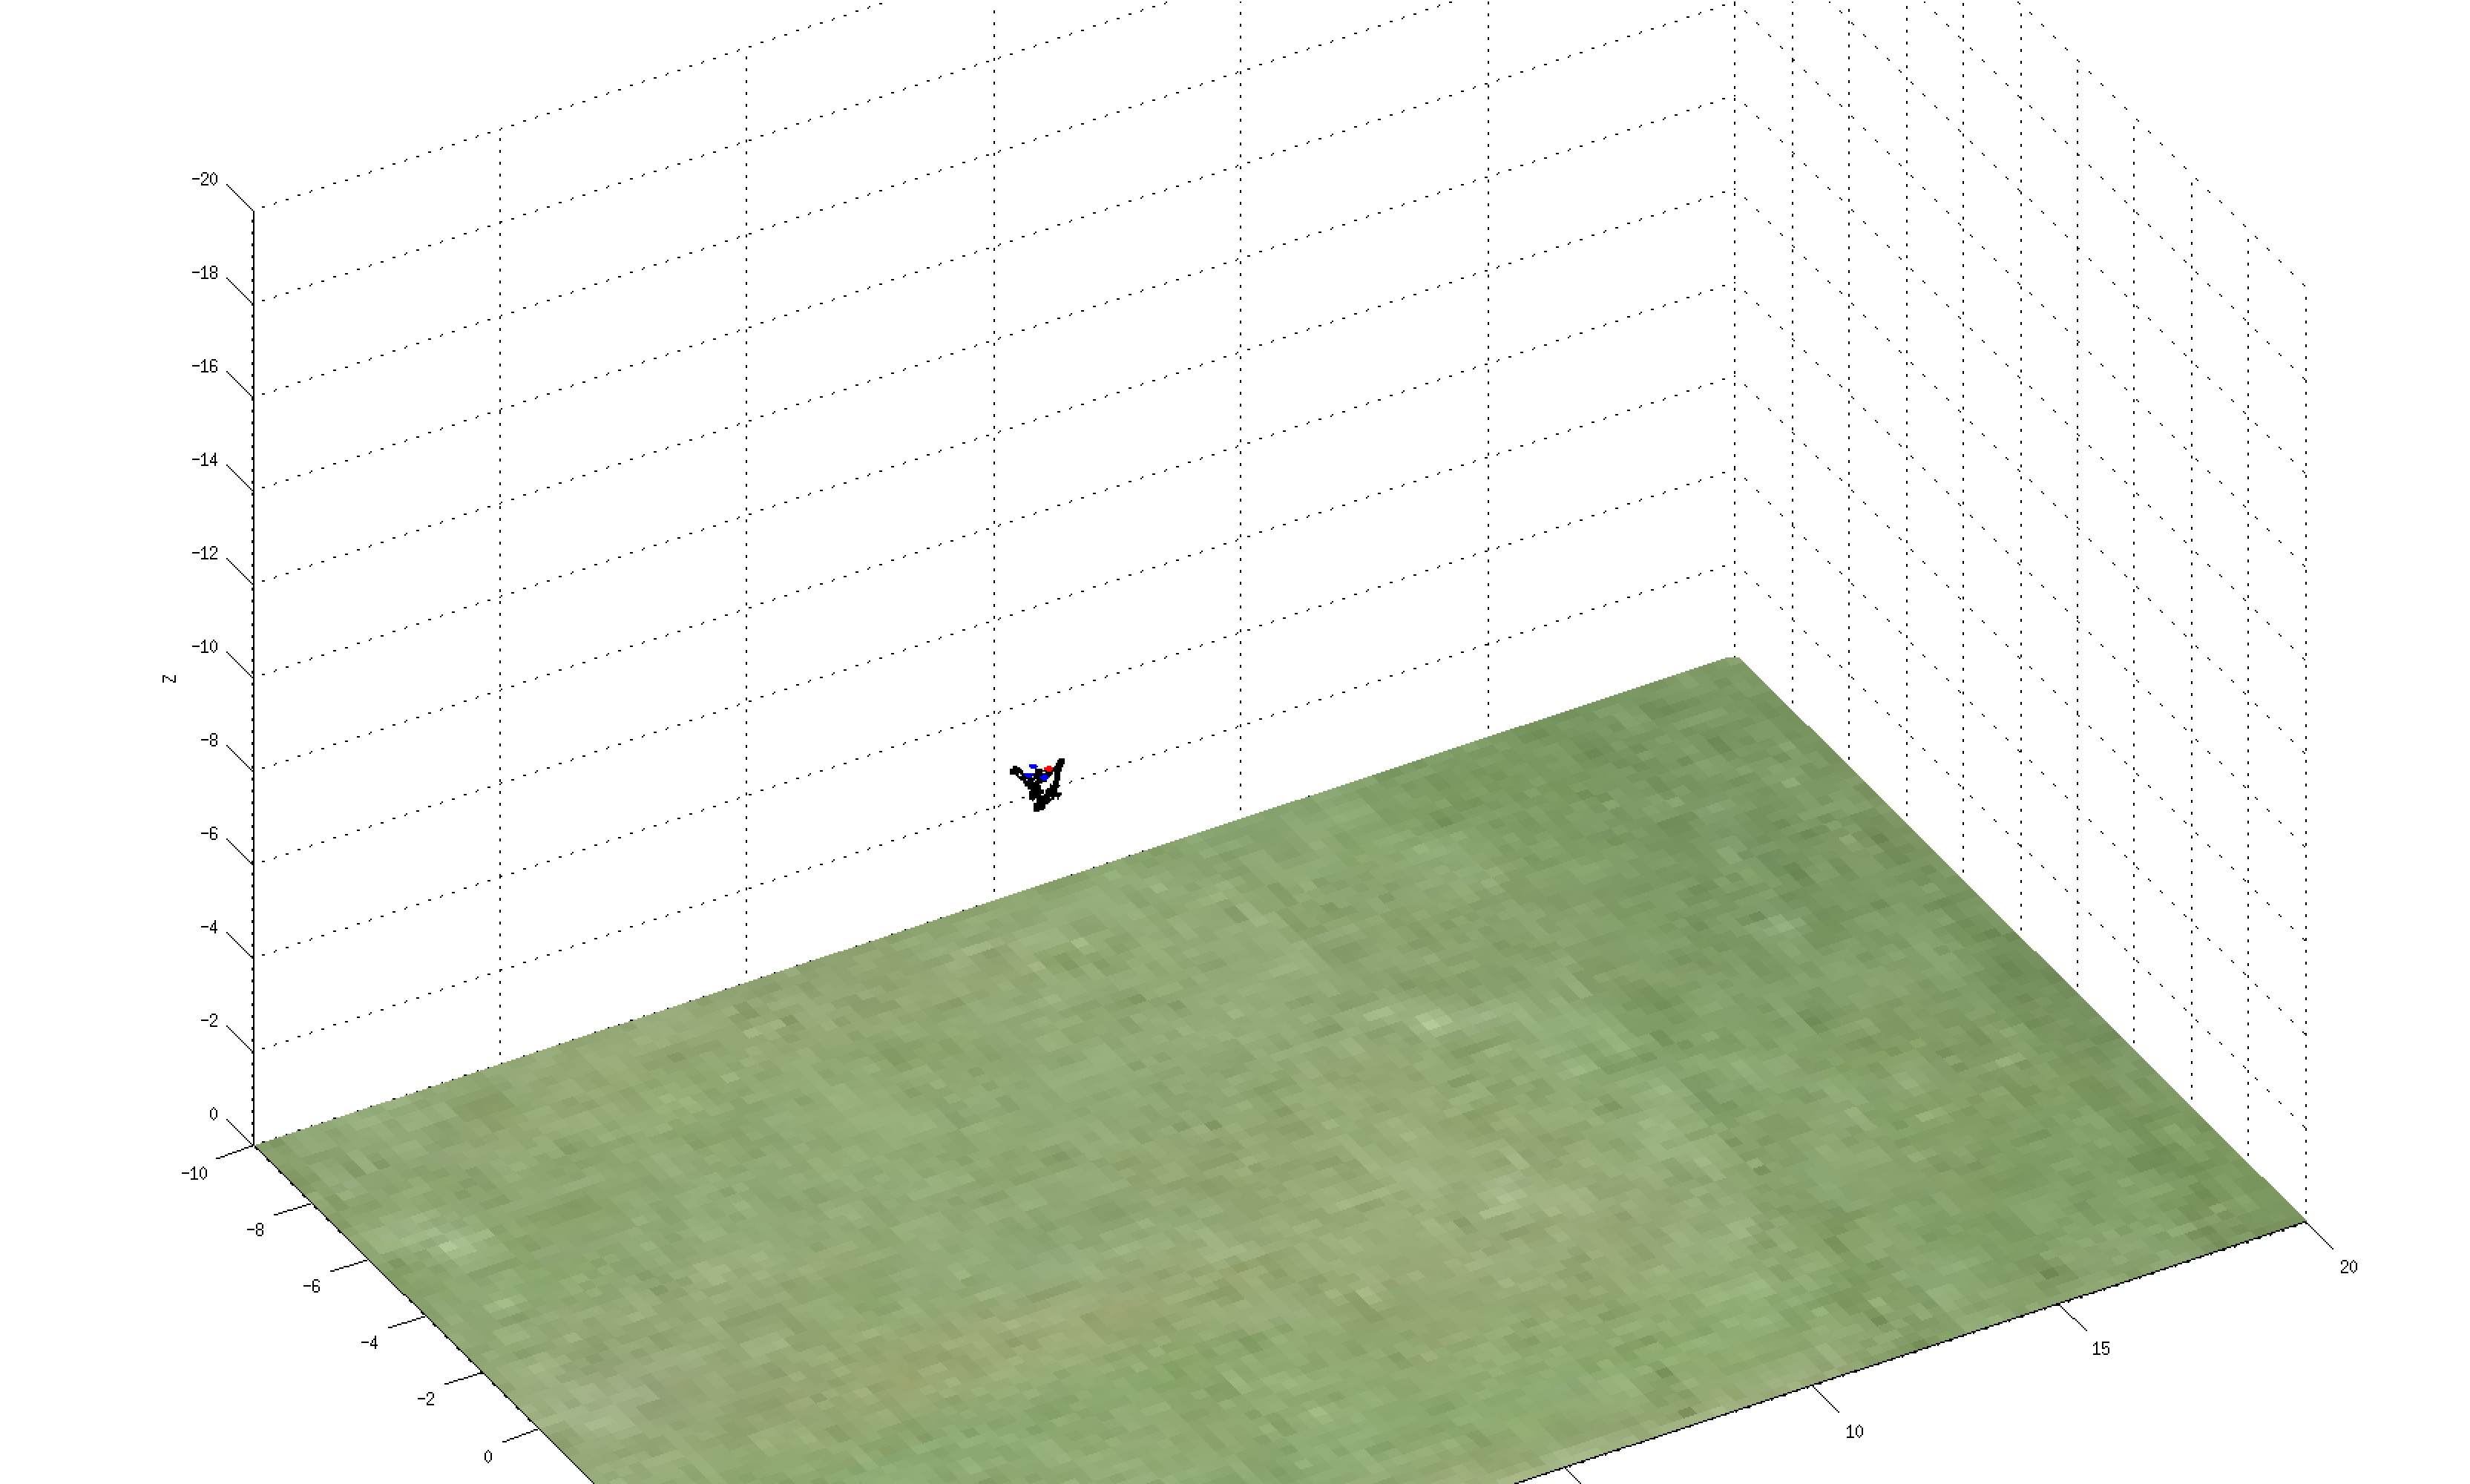
\includegraphics[width=18cm]{main.eps}
 \caption{Typical main output figure}
\end{center}
\end{figure}

\section*{Exercise 1:\\Creating a new project}

A new qrsim simulation is usually composed of at least three files:
\begin{itemize}
 \item a main scripts that control the execution of the simulation;
 \item a task file that define the configuaration for the environment objects;
 \item a platform configuration file that defines the setting for the platform sensors.
\end{itemize}
Create a new directory in a location of your choice\footnote{Using qrsim within a project only requires to have the \texttt{sim} directory in the class path therefore you have complete freedom of choosing where to keep your projects.} and copy into it the files:
\begin{itemize}
 \item \texttt{example/main.m}
 \item \texttt{sim/tasks/TaskKeepSpot.m}
 \item \texttt{sim/platforms/pelican\_config.m}
\end{itemize}
Since we will be modifying these files in the following exercises it makes sense to rename them to something more meaningful; let's rename \texttt{TaskKeepSpot.m} to \texttt{TaskTutorial.m} and \texttt{pelican\_config.m} to \texttt{pelican\_config\_tutorial.m}.

Of course now we need to update the files that reference souch scripts, this will give us the chance to see what references what, within one of our projects.
We start by editing \texttt{main.m}:
\begin{itemize}
 \item line 8: update \texttt{addpath('../sim:../controllers');} to point to the right directories in your machine. Note that is is the only thing needed to make use of qrsim in your project.
 \item line 14: update \texttt{state = qrsim.init('TaskKeepSpot');} to reference the renamed task \texttt{TaskTutorial.m}. Note that this is the only location in which a task is referenced.
\end{itemize}  
Now, since \texttt{TaskTutorial.m} is a Matlab class, its filename needs to match the class name\footnote{If you are not familiar with object-oriented programming in Matlab you can find more informations here: \url{http://www.mathworks.co.uk/help/techdoc/matlab_oop/ug_intropage.html}}, we therefore need open \texttt{TaskTutorial.m} in the file editor and do the following:
\begin{itemize}
 \item line 1: replace \texttt{classdef TaskKeepSpot<Task} with \texttt{classdef TaskTutorial<Task}
 \item line 28: replace \texttt{obj = TaskKeepSpot(state)} with \texttt{obj = TaskTutorial(state)}.
\end{itemize}
Finally if we look at the bottom of the method \texttt{init()} defined in \texttt{TaskTutorial.m} (line 102) we can see that the script \texttt{pelican\_config} is indicated as the configuration file that should be used for platform 1. Obviously we want to change this to \texttt{pelican\_config\_tutorial} so that the configuration file that we have in the current project is used instead.

At this point, we are done with creating a new project. You can now test that the modifications we just applied did not break the project; simply run \texttt{main.m} and you should see the same output you got in Exercise 0. 


\section*{Exercise 2:\\Familiarise with \texttt{QRSim} and platforms objects}

We now have a look in more detail at the file \texttt{main.m}; open it in your matlab editor. 
This script implements what is one of the simplest way of running a simulation using qrsim; nevertheless it shows the three foundamental steps that are always needed when running a simulation:
\begin{itemize}
 \item line 11: \texttt{qrsim = QRSim()}  creation of a simulation object; \\
  this instruction takes care of initializing the path variables correctly and creates (but does not initialize) the data structure that maintains the simulation state. 
 \item line 14: \texttt{state = qrsim.init('TaskTutorial')} initialisation of the simulation;\\
  the setting specified in the task are used to instantiate the required platform and environment objects, and subsequently to initialised them to the required state. After calling \texttt{init} the simulator is in a valid state and the simulation time \texttt{state.t} is equal to zero.
 \item line 35: \texttt{qrsim.step(U)} stepping the simulator;\\
  this command first updates the enviroment objects and then applies to each platform the given input \texttt{U} (where \texttt{U} is a matrix with a number of columns equal to the number of platforms\footnote{Use \texttt{doc Pelican} to see details about meaning and ranges of the contrul inputs.}). At completion the simulation time had advanced of \texttt{state.DT}.  
\end{itemize}
From the description just given one can understand that calling \texttt{step} only makes sense after the simulation is created and initialized to a valid state. 
In our example the simulator is stepped within a for loop since we want to run the task for \texttt{N} steps but is rather obvious that this does not need to be the case; once the simulation object is initialized the step method can be called in whatever fashion is more convenient to the user.

Now that is more clear what the \texttt{main.m} script is doing, modify it in order to produce a time plot of the true and of the estimated platform position. Use a 3 by 1 subplot so that you can plot each of the three (x,y,z) components independently.   
In a real platform the altitude estimated using the barometric altimeter is often more accurate than the one produced by the GPS receiver for this reason you will plot the former instead of $p_x$ in your plots.
Once you obtained the plots have a good look at the true and estimated variables, what do you notice?

The following methods defined in the class \texttt{Pelican} (accessible as \texttt{state.platforms{1}.getX()}) will be useful to carry out the above:
\begin{itemize}
 \item \texttt{getEX()} returns the estimated state (noisy) state;
 \item \texttt{getX()} returns the true state (noiseless) state;
 \item \texttt{getEXasX()} returns the estimated state (noisy) formatted as the noiseless state;
 \item \texttt{isValid()} returns true if the state is valid; the state can become not valid if the uav exits the flying area (e.g. hits the ground) or if two uavs collide;
\end{itemize}
use the command \texttt{doc Pelican} to have more details about the format of the returned data\footnote{The commands \texttt{getEX(), getX()} and \texttt{getEXasX()} all accept intervals as argument (e.g. \texttt{getEX(1:3)}); this provides an easy way to query only for the variables of interest.}.

Note:
in order to update the figure containing the 3D visualization the simulator needs to redefine the current window, this might interfere with your plot.
In order to avoid that you can store the handles of your plots before the beginning of the for loop and then update the plot inside the loop by setting the \texttt{YData} property of each plot.

\section*{Exercise 3:\\Modify task and platform settings}

So far we kept unchanged the settings of both the environment and of the platforms in our task, in this exercise we will explore the effects of changing such parameters.

Open the file \texttt{TaskTutorial.m} and look at the function \texttt{init()}, you will see that the parameters are divided into sections corresponding to the various environment objects. Also note how we use a nested naming scheme in order to specify the properties of each object.
Most of the objects have the property \texttt{on} which allow to enable or disable the module in question and some have a parameter \texttt{dt} that defines the update rate.

Try out some of the following changes \textsf{in turn}, and look at the resulting behaviour of the helicopter (remember to save the task file before re-running \texttt{main.m}): 
\begin{itemize}
 \item set \texttt{taskparams.seed} to a number different from $0$ and run the simulation twice. What do you notice about the flight path of the helicopter?
 \item set \texttt{taskparams.display3d.on} to $0$; the simulation will run withoud 3D display. Did you notice any change in simulation speed?
 \item change the values of \texttt{taskparams.environment.area.limits}, you will see the 3D area changing accordingly\footnote{If you change the area so that the starting position of the helicopter is outside the flying volume the simulation won't run!}.
 \item try to set \texttt{taskparams.environment.gpsspacesegment.on} to $0$, what happens? We will see later why this is the case.
 \item set \texttt{taskparams.environment.wind.on} to $1$, and run the simulation twice with different values of \texttt{taskparams.environment.wind.direction}. You should see a clear effect on the helicopter flight pattern.
 \item experiment with different initial values for the platform state \texttt{taskparams.platforms(1).X}, note that you can also define the initial velocities by specifying an initial state of lenght 12.
\end{itemize}

Let's now continue by experimenting with the platform settings and therefore editing the file \texttt{pelican\_config\_tutorial.m}.
Immediately one can see that the file uses the same naming convention that we have seen for the environment object parameters. 
Even in this case is intructive to make changes to the setting and compare the output of the simulator. We suggest to try some of the following:
\begin{itemize}
 \item set \texttt{sensors.gpsreceiver.on} to $0$ and run the simulation; the GPS receiver noise is now off. What happens to the plots of estimated and true position that we set up in Excercise 2?
\item if you now go back to \texttt{TaskTutorial} and retry setting \texttt{environment.gpsspacesegment.on} to $0$; you should now be able to run the simulations without any error.
\item set \texttt{sensors.ahars.on} to $0$ to turn off any noise in the inertial sensors; this should be clearly visible if you plot true and estimated angles (or angular velocities). 
\item set \texttt{aerodynamicturbulence.on} to $0$; is the flight behaviour changed?
\item set \texttt{aerodynamicturbulence.on} and \texttt{sensors.gpsreceiver.on} both to $0$; do you see a drastic improvement in the capability of the helicopter in keeping station?
\end{itemize}


\section*{Exercise 4:\\Set and reset the platform state}

We have seen how changing the initial platform state in the \texttt{pelican\_config\_tutorial.m} is very straightforward but is often necessary to be able to save, set and reset the platform state at runtime.

  
set / reset state


\section*{Exercise 5:\\Using predifined PID controllers}


controllers


\section*{Exercise 6:\\Defining a task reward}

A task is defined not only by the configuration of platforms and environment objects but also by the  objective that needs to be achieved.


Is important to point out that while defining rewards within a task is very handy, this is by no means something necessary to perform simulations using qrsim. In facts the \texttt{updateReward()} and \texttt{reward()} methods of a task can simply be left empty if not needed.

\section*{Exercise 7:\\Working with several helicopters}

Up until now we only considered one single helicopter, however qrsim can readily deal with more than one platform.
Let's try to modify the task file and \texttt{main.m} to handle 10 different helicopters; to do so you will need to:
\begin{itemize}
 \item modify the platforms section of \texttt{TaskTutorial.m} to define \texttt{configfile} and initial state \texttt{X} for each of the platform. You can easily do this with a for loop but make sure that the initial position of the platform are sufficiently far apart otherwise they would be deemed in collision.
\item modify \texttt{main.m} so that ten different waypoints and ten different pid controller are created instead of only one of each. In the for loop use each of the ten pids to compute the control input for the respective helicopter. Remember to bundle up the control commands of each platform as columns of the matrix \texttt{U} so you can pass it to the step method of qrsim.
\end{itemize}
If you get stuck you can have a look in the directory \texttt{example}, the file \texttt{main10.m} shows a possible solution to this excercise.

Now that you have several helicopters in your simulation you can play around with the parameter \texttt{collisionDistance} in \texttt{pelican\_config\_tutorial.m} and verify that if two paltforms are closser than the collision distance both will be deemed had having an invalid state.



%\bibliography{manual}
%\bibliographystyle{plain}
\end{document}          
